\documentclass[12pt]{article}

\usepackage[dvips]{graphics}
\usepackage{latexsym,amssymb}
\usepackage[colorlinks,backref,bookmarks=true]{hyperref}

\addtolength{\textwidth}{1.7cm}%
\addtolength{\textheight}{5.5cm}%
\addtolength{\hoffset}{-1.5cm}%
\addtolength{\voffset}{-2.0cm}%

\newcommand{\topic}[1]{\vspace{.15in}\LARGE \textbf{#1} \vspace{.15in} \normalsize }
\newcommand{\workspace}[1]{\vspace{#1in}}

\newcommand{\norm}[1]{\left\|\,#1\right\|}
\newcommand{\pnorm}[2]{\left\|\,#1\,\right\|_{#2}}
\newcommand{\absv}[1]{\left|\,#1\right|}
\newcommand{\bigo}[1]{\mathcal{O}(#1)}
\newcommand{\keyw}[1]{\emph{\textbf{#1}}}


\usepackage{amssymb}
% \pagestyle{empty}

\begin{document}

\begin{center}
\topic{The Matlab Postprocessing Toolkit (MPT) User Manual}
\end{center}

The MPT user manual first lists all Matlab functions associated with each edge detection and postprocessing algorithm. For each algorithm there is also an example script that demonstrates how the Matlab function can be used that implements the algorithm.   For each example script, there is a figure that shows the graphical output of the script.

\section{Edge Detection}

\begin{figure}[tbh]
   \centering
      \scalebox{0.7}{\includegraphics{edgeDetectCheby1.eps}}
 \caption{Un-enhanced and enhanced edge detection data produced by edgeDetectChebyshev\_example.m using the exponential concentration factor. The following edge detection parameters were used: $Q=2$, $J=30$, and $\eta=2$.
          } \label{fig:edgeDetect}
 \end{figure}

Matlab files: (Note: the inputs and outputs of all the MPT functions are documented in the m-files)
\begin{enumerate}
    \item edgeDetectChebyshev.m
    \item edgeDetectFourier.m
    \item edgeDetectChebyshev\_example.m - The example applies the
    edge detection routine to the Chebyshev approximation of the
    function
\begin{equation}
 f(x)= \left\{
\begin{array}{ll}
  \cos(\pi x/2) & x < -0.5 \\
  x^3 - \sin(3\pi x/2) & -0.5 \leq x \leq 0.5   \\
  x^2 + 4x^3 - 5x  & x > 0.5
\end{array}
\right. \label{function:2discont}
\end{equation}
     The output is shown in figure  \ref{fig:edgeDetect}.
\end{enumerate}

\section{Spectral Filter}

\begin{figure}[tbh]
   \centering
      \scalebox{0.65}{\includegraphics{fourierGibbs.eps}\includegraphics{chebyshevGibbs.eps}}
 \caption{Spectral approximation of function (\ref{function:sincos}) vs. the exact function.  The function is known at $N=200$ interpolation sites and the interpolant is evaluated at $M=298$ evenly spaced points. Left: Fourier.  Right: Chebyshev.
          } \label{fig:gibbsExample}
 \end{figure}

The Gibbs phenomenon is illustrated in figure \ref{fig:gibbsExample} for both the Fourier and Chebyshev approximation of the function
\begin{equation}\label{function:sincos}
    f(x) = \chi_{[-0.5,0.5]} \ast \sin[\cos(x)]
\end{equation}
that will be used throughout to demonstrate the software.


\begin{figure}[tbh]
   \centering
      \scalebox{0.7}{\includegraphics{filterFourier1.eps}\includegraphics{filterFourier2.eps}}
 \caption{Output produced by spectralFilter\_example.m. Left: Function (\ref{function:sincos}), and the filtered Fourier approximation
 of the function.  Right: Error of the Fourier approximation and the
 reduced error of the filtered approximation.
          } \label{fig:spectralFilter}
 \end{figure}


Matlab files:
\begin{enumerate}
    \item spectralFilter.m
    \item spectralFilter\_example.m -
    The example calculates the Fourier approximation of the function (\ref{function:sincos})
   and the filtered approximation using the fourth-order Vandeven
   filter.  The output is shown in figure \ref{fig:spectralFilter}.
   The right image shows the increased accuracy of the filtered
   approximation away from the discontinuity.  The oscillatory Fourier approximation is in
   the left image of figure \ref{fig:gibbsExample}.
    \item filterFourier.m
    \item filterFourier2d.m
    \item filterChebyshev.m
    \item filterChebyshev2d.m
\end{enumerate}

\section{Digital Total Variation Filtering}

\begin{figure}[tbh]
   \centering
      \scalebox{0.65}{\includegraphics{dtvFourier1.eps}\includegraphics{dtvFourier2.eps}}
 \caption{Output produced by dtvFilter\_example.m. Left: Function (\ref{function:sincos}) and the DTV postprocessed Fourier approximation.  Right: Error of the Fourier approximation and the
 reduced error of the DTV postprocessed approximation.
          } \label{fig:dtvFilter}
\end{figure}

Matlab files:
\begin{enumerate}
  \item digitalTotalVariationFilter.m - 1d non-periodic
  \item digitalTotalVariationFilterPeriodic.m - 1d periodic
  \item digitalTotalVariationFilter\_2d.m - 2d non-periodic using $N_\alpha^4$
  \item digitalTotalVariationFilter\_2d\_8.m - 2d non-periodic using $N_\alpha^8$
  \item digitalTotalVariationFilterPeriodic\_2d.m - 2d periodic using $N_\alpha^4$
  \item digitalTotalVariationFilterPeriodic\_2d\_8.m - 2d periodic using $N_\alpha^4$
  \item fourierDTV\_example.m - The example postprocesses the Fourier approximation of function (\ref{function:sincos})
  using the DTV filter (digitalTotalVariationFilterPeriodic.m) with $\lambda = 10$ and $100$ time steps.  The output is shown in figure \ref{fig:dtvFilter}. The oscillatory Fourier approximation is in
   the left image of figure \ref{fig:gibbsExample}.
  \item periodic\_dtv\_example\_2d.m - The example postprocesses the Fourier approximation of the function
\begin{equation}
 f(x)= \left\{
\begin{array}{ll}
  1 & x^2 + y^2 \leq \frac{1}{4} \\
  0 & \mbox{ otherwise }
\end{array}
\right. \label{function:circle2d}
\end{equation}
   using the DTV filter (digitalTotalVariationFilterPeriodic.m) with $\lambda = 10$ and $100$ time steps.  The output is shown in figure \ref{fig:dtvExample2d}.  The function is sampled on a $64 \times 64$ grid and evaluated on a uniformly spaced $98 \times 98$ grid.
\end{enumerate}

\begin{figure}[tbh]
   \centering
      \scalebox{0.65}{\includegraphics{2dDtv1.eps}\includegraphics{2dDtv2.eps}}
 \caption{Output produced by periodic\_dtv\_example\_2d.m. Left: Fourier approximation of function (\ref{function:circle2d}).  Right: The DTV postprocessed Fourier approximation using digitalTotalVariationFilterPeriodic\_2d.m.
          } \label{fig:dtvExample2d}
 \end{figure}
 
\section{Rational Reconstruction}

Matlab files:
\begin{enumerate}
  \item fourierPade.m
  \item chebyshevPade.m
  \item chebyshevPade\_example.m - Figure \ref{fig:chebyPade} shows the output of the chebyshevPade\_example.m which applies chebyshevPade.m with $M=14$ to postprocess function (\ref{function:sincos}).  The oscillatory Chebyshev approximation is in the right image of figure \ref{fig:gibbsExample}.
\end{enumerate}

\begin{figure}[tbh]
   \centering
      \scalebox{0.65}{\includegraphics{chebyshevPade1.eps}\includegraphics{chebyshevPade2.eps}}
 \caption{Output produced by chebyshevPade\_example.m. Left: Function (\ref{function:sincos}), and the postprocessed approximation of the function.  Right: Error of the Chebyshev approximation and the
 reduced error of the postprocessed approximation.
          } \label{fig:chebyPade}
 \end{figure}
 
\section{Gegenbauer Reprojection}

\begin{figure}[tbh]
   \centering
      \scalebox{0.65}{\includegraphics{grpFourier1.eps}\includegraphics{grpFourier2.eps}}
 \caption{Output produced by fourierGRP\_example.m. Left: Function (\ref{function:sincos}) and the GRP postprocessed Fourier approximation (visually indistinguishable).  Right: Error of the Fourier approximation and the
 reduced error of the postprocessed GRP approximation.
          } \label{fig:fourierGrpExample}
 \end{figure}
 
 Matlab files:
\begin{enumerate}
  \item grp.m
  \item fourierGRP\_example.m - see figure \ref{fig:fourierGrpExample}.  The example has three smooth subintervals $\Omega_1 = [-1,-0.5)$, $\Omega_2 = (-0.5,0.5)$, and $\Omega_3 = (0.5,1]$.  The example used the following GRP parameters: $m_1 = m_2 = m_3 = 13$, $\lambda_1 = 4$, $\lambda_2 = 7$, and $\lambda_3 = 4$.  The oscillatory Fourier approximation is in the left image of figure \ref{fig:gibbsExample}.
  \item chebyshevSV\_eulerDensity\_grp.m - Applies the GRP to postprocess the $N=128$ Chebyshev spectral viscosity approximation of the density profile of Sod's problem \cite{Sod78} for the Euler equations
  of gas dynamics. The output is in figure \ref{fig:eulerDensityGrpExample}.  The example has five smooth intervals: $\Omega_1 = [-1,-0.4456)$,  $\Omega_2 = (-0.4456,-0.0222)$, $\Omega_3 = (-0.0222,0.3461)$, $\Omega_4 = (0.3461,0.6606)$, and $\Omega_5 = (0.6606,1]$. The following GRP parameters were used in the example:  $m_1=4$, $m_2=12$, $m_3=4$, $m_4=4$, $m_5=4$, $\lambda_1=5$, $\lambda_2=6$, $\lambda_3=6$, $\lambda_4=4$, and $\lambda_5=4$.
\end{enumerate}

\begin{figure}[tbh]
   \centering
      \scalebox{0.7}{\includegraphics{eulerDensity128.eps}\includegraphics{eulerDensityError.eps}}
 \caption{Output of chebyshevSV\_eulerDensity\_grp.m.  Left: Chebyshev spectral viscosity and GRP postprocessed Euler density solution at time t = 0.4. Right: Error of the postprocessed solution.
          } \label{fig:eulerDensityGrpExample}
 \end{figure}

\section{Freud Reprojection}

Matlab files:
\begin{enumerate}
  \item frp.m
  \item freudPolynomials.m
  \item fourierFreud\_example.m - The script uses the FRP to postprocess the oscillatory Fourier approximation in the left image of figure \ref{fig:gibbsExample}. The results are shown in figure \ref{fig:fourierFreudExample}.  The following FRP parameters were used: $m_1 =2$, $m_2 = 12$,  $m_3= 2$, $\lambda_1 = 7$, $\lambda_2 = 11$, and $\lambda_3 = 7$.
\end{enumerate}

\begin{figure}[tbh]
   \centering
      \scalebox{0.65}{\includegraphics{frpFourier1.eps}\includegraphics{frpFourier2.eps}}
 \caption{Output produced by fourierFreud\_example.m. Left: Function (\ref{function:sincos}) and the FRP postprocessed Fourier approximation (visually indistinguishable).  Right: Error of the Fourier approximation and the
 reduced error of the postprocessed FRP approximation.
          } \label{fig:fourierFreudExample}
 \end{figure}
 
\section{Inverse Reprojection}

Matlab files:
\begin{enumerate}
  \item inverseReprojection.m
  \item fourierIPRM\_example.m - This script uses the IPRM to postprocess the oscillatory Fourier approximation in the left image of figure \ref{fig:gibbsExample}. The output is shown in figure \ref{fig:fourierIprmExample}.  The following IPRM parameters were used: $m_1 = 2$, $m_2=6$, and $m_3=2$.
\end{enumerate}

\begin{figure}[tbh]
   \centering
      \scalebox{0.65}{\includegraphics{iprmFourier1.eps}\includegraphics{iprmFourier2.eps}}
 \caption{Output produced by fourierIPRM\_example.m. Left: Function (\ref{function:sincos}) and the IPRM postprocessed Fourier approximation.  Right: Error of the Fourier approximation and the reduced error of the postprocessed IPRM approximation.
          } \label{fig:fourierIprmExample}
 \end{figure}



\end{document}
